\head{Ноябрь}{Листок 4. Теория чисел. Уровень 3+.}

\begin{thm}Докажите, что
    \par
    а)~число тогда и только тогда делится на 4, когда две его последние цифры образуют число, \\ делящееся на 4.
    \par
    б)~число тогда и только тогда делится на 8, когда число, составленное из трех последних его цифр делится на 8.
\end{thm}



{
\setlength{\intextsep}{0pt}
\begin{figure}[h]
\begin{minipage}[h]{0.72\linewidth}\setlength{\parindent}{1.5em}
\begin{thm}
    Попробуйте сформулировать и доказать признаки делимости на 7 и на 13.
    \\ 
    {\footnotesize\textit{(\underline{Подсказка}: $1001=7\times11\times13$)}}
\end{thm}
    \begin{thm}
    Перед боем с белогвардейцами у Василия Ивановича и Петьки было поровну патронов. Василий Иванович израсходовал в бою в 8 раз меньше патронов, чем Петька, а осталось у него в 9 раз больше патронов, чем у Петьки. Докажите, что изначально количество патронов у Василия Ивановича делилось на 71. 
    \end{thm}
\end{minipage}
\hfill
\begin{minipage}[h]{0.25\linewidth}
    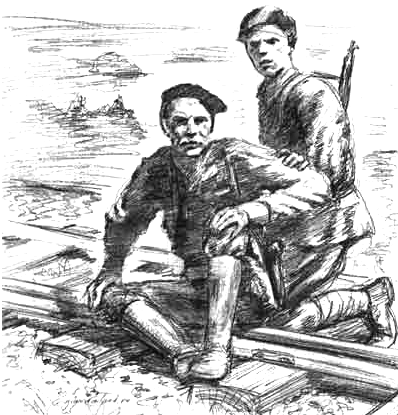
\includegraphics[width=0.9\columnwidth]{./img/soldat}
\end{minipage}

\end{figure}
}

    \begin{thm}
    Автоматический хозрасчётный калькулятор предоставляет следующие услуги:
    \par 
    I)~Умножение имеющегося числа на три за 5 коп.; 
    \par
    II)~Прибавление к имеющемуся числу четырёх за 2 коп. 
    \par
    Число 1 вводится бесплатно. Какую наименьшую сумму нужно потратить, чтобы получить число 2012?
\end{thm}

\begin{thm}$^{\ast}$
Назовём автобусный билет с шестизначным номером счастливым, если сумма цифр его номера делится на 7. Могут ли два билета подряд быть счастливыми?
\end{thm}
{
\setlength{\intextsep}{0pt}
\begin{figure}[h]
\begin{minipage}[h]{0.72\linewidth}\setlength{\parindent}{1.5em}
    \begin{thm}$^{\ast}$
    Шайка разбойников отобрала у купца мешок с монетами. Каждая монета стоит целое число грошей. Оказалось, что какую монету не отложи, оставшиеся монеты можно поделить между разбойниками так, что каждый получит одинаковую сумму. Докажите, что число монет без одной делится на число разбойников в шайке.
    \end{thm}
\end{minipage}
\hfill
\begin{minipage}[h]{0.25\linewidth}
    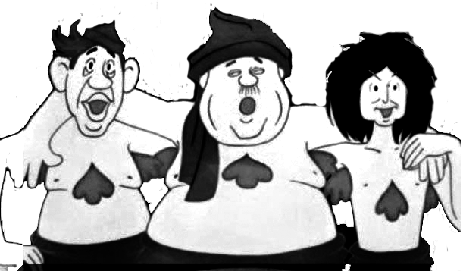
\includegraphics[width=0.9\columnwidth]{./img/razboi}
\end{minipage}
\end{figure}
}